\section{Study of $R_{NL}$}
Unfortunately \ref{eq:rnlk} doesn't have an analytic Fourier transform. If there are no topological effect, so $\tan (\theta_{VH})=0$, it can be solved analytically.

\begin{equation}
    R_{NL}(x)=\frac 2{\sigma_c}\int_{-\infty}^{+\infty}
    \frac{\tanh (kW/2)}k \frac {dk}{2\pi}=
    -\frac{2\rho}\pi\ln\bigg |\tanh \Big(\frac{\pi x}{2W}\Big)\bigg |
    \label{eq:ohmic signal2}
\end{equation}
This is the purely ohmic nonlocal signal that we have talked about in \ref{eq:ohmic signal}.

However if we are going to explore topological materials we cannot set $\tan (\theta_{VH})=0$, rhis means that we'll have to explore equation \ref{eq:rnlk} in regimes where it is approximately equal to a function that admits an analytic Fourier transform.

Let's look at the graph of the $R_{NL}(k)$ before doing any approximations:
\begin{figure}[h!]
    \centering
    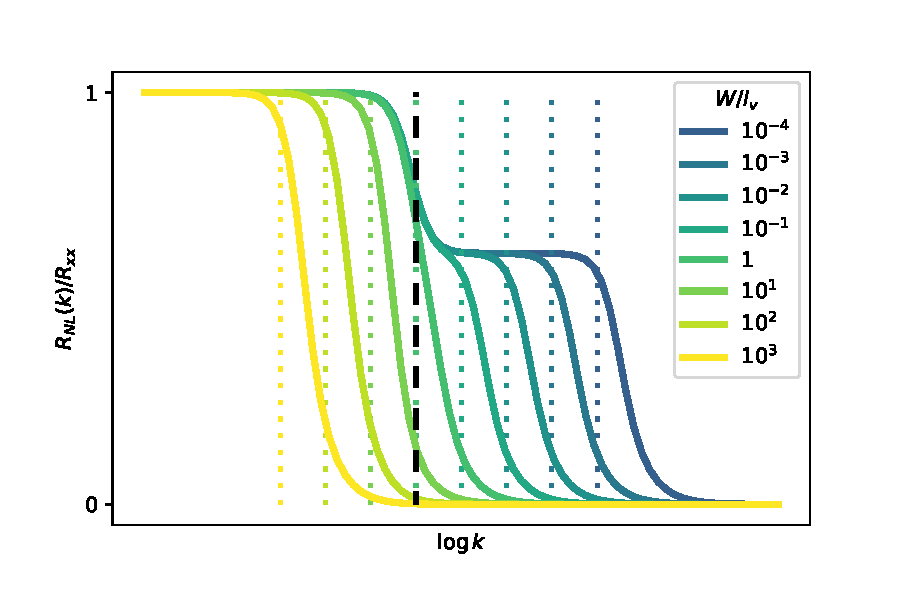
\includegraphics[width=\linewidth]{Immagini/rnl/widths.pdf}
    \caption{$R_{NK}(k)$ for several values of $W/l_v$. The dashed black line represents where $k=1/l_v$, the colored dashed line represents where $k=1/W$}
    \label{fig:RNLk}
\end{figure}
As you can see from the figure \ref{fig:RNLk} if $W\gg l_v$ we have a single bell like function with the width of the bell being $\approx 1/W$. If $W\ll l_v$ we have a double-bell function, where the first bell has a height of $1$ and a width of $1/l_v$, and the second one has a shorter height. To evaluate the precise height we just need to set $l_v^{-1}\ll k \ll W^{-1}$ in equation \ref{eq:rnlk}, this gives us 


\[
R_{NL}(l_v^{-1}\ll k \ll W^{-1})\approx \frac{R_{xx}}{1+\tan^2(\theta_{VH})}    
\]
Where $R_{xx}=\frac{W}{\sigma_{xx}}$

So, if we have $l_v\ll W$ or $\tan(\theta_{VH})\ll 1$ (or both) we have a single bell structure. Incidentally these are the conditions to NOT have topological effects, so the less visible the double bell is, the less visible the topological effects are. We'll also see later how one of the bell represents the ohmic nonlocal signal, while the other represents the topological nonlocal signal. 


Let's start by exploring $k\ll l_v^{-1},W^{-1}$. This will tell us how the function behaves for $x\gg l_v,W$. In this regime 

\begin{equation}
    \omega(k)\approx \frac 1{l_v}\bigg[1+\frac{(kl_v)^2}2\bigg]\quad\quad
    \coth (kW/2)\approx \frac 2{kW} + \frac{kW}6
\end{equation}
Plugging this into equation \ref{eq:rnlk} we have that $R_{NL}(k)\approx$
\begin{equation}
    \frac 2{\sigma_c}\frac 1 {l_vk}\Bigg[
        \frac 1{l_v}\bigg(1+\frac{k^2l_v^2}{2}\bigg)\bigg(\frac 2{kW} + \frac{kW}6\bigg)+
        \frac{k\tan^2(\theta_{VH})}{\tanh(W/2l_v)} + o(k^2)
    \Bigg]^{-1}
\end{equation}
With some mathematical manipulation it can be shown that it is equal to 
\begin{equation}
    R_{NL}(k\ll l_v^{-1},W^{-1})=
    \frac W{\sigma_c}\frac 1{1+L_v^2k^2} + o(k^3)
    \label{eq:lorentz1}
\end{equation}
where the renormalized valley diffusion length $L_v^2$ is 
\begin{equation}
    L_v^2 = l_v^2+\frac {W^2}{12} +\frac{l_vW}2 \frac{\tan^2(\theta_{VH})}{\tanh(W/2l_v)}
\end{equation}
Now we do the Fourier transform of equation \ref{eq:lorentz1} ignoring the $o(k^3)$ term to get the behavior of $R_{NL}(x\gg l_v,W)$
\begin{equation}
    R_{NL}(x\gg l_v,W)=\mathcal F^{-1}R_{NL}(k\ll l_v^{-1},W^{-1}) 
    \label{eq:rxg}
\end{equation}
That is equal to 

\begin{equation}
    \frac W{\sigma_c}\int_{-\infty}^{+\infty}
    \frac 1{1+L_v^2k^2}
    \frac {dk}{2\pi}=
    \frac{W\rho}{2L_v}e^{-\frac{|x|}{L_v}}
\end{equation}
So,
\begin{equation}
    R_{NL}(x\gg l_v,W)=\frac{W\rho}{2L_v}e^{-\frac{|x|}{L_v}}
    \label{eq:rxl}
\end{equation}


Now we are going to study what happens for $k\gg l_v^{-1}$, in this case $\omega(k) \approx k$, So

\begin{equation}
    R_{NL}(k\gg l_v^{-1})=\frac 2{\sigma_c}\frac{\tanh}k\bigg(\frac{kW}2\bigg)\frac 1{1+\tan^2(\theta_{VH})}
\end{equation}
it's Fourier transform is
\begin{equation}
    R_{NL}(x\ll l_v)=-\frac 2{\pi\sigma_c}\frac 1{1+\tan^2(\theta_{VH})} \ln\bigg |\tanh \Big(\frac{\pi x}{2W}\Big)\bigg |
\end{equation}
This last equation is $1+\tan^2(\theta_{VH})$ smaller to the one for the purely ohmic nonlocal signal (eq. \ref{eq:ohmic signal2})

Now let's see how these equations fear in practice
\begin{figure}[h!]
    \centering
    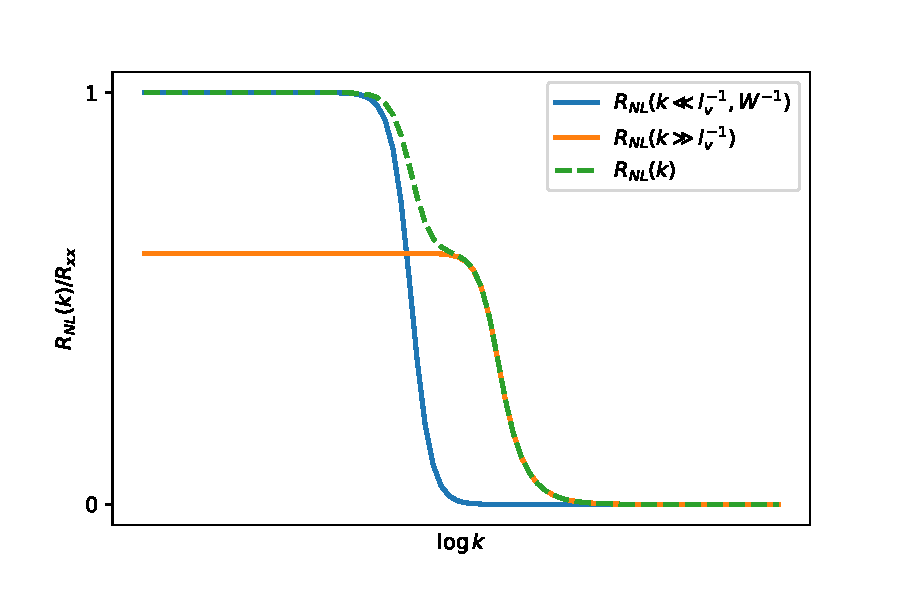
\includegraphics[width=\linewidth]{Immagini/rnl/2approx.pdf}
    \caption{For this example $l_v=20W$}
    \label{fig:rnl2approx}
\end{figure}
As you can see from figure \ref{fig:rnl2approx} the two approximations work pretty well, except in the neighborhood where $k\approx l_v^{-1}$. But what we really care about is $R_{NL}(x)$.\\
If we plot $R_{NL}(x\gg l_v,W)$ (eq. \ref{eq:rxg}) and $R_{NL}(x\ll l_v)$ (eq. \ref{eq:rxl}) alongside the numerical Fourier transform of $R_{NL}(k)$ \ref{eq:rnlk} we get figure \ref{fig:rnlx2approx}

\begin{figure}[h!]
    \centering
    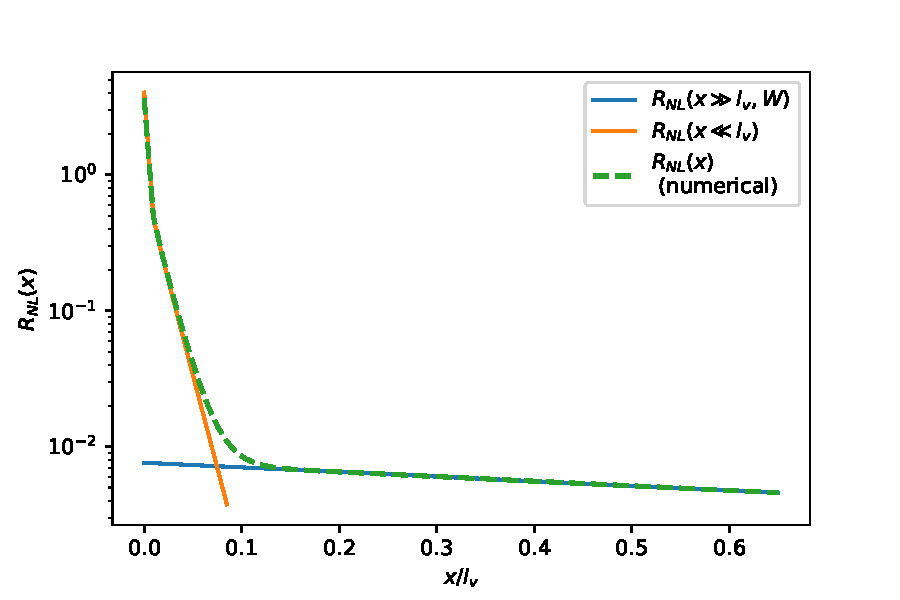
\includegraphics[width=\linewidth]{Immagini/rnl/x2approx.pdf}
    \caption{The parameters for this graph are exactly the same for the previous graph (figure \ref{fig:rnl2approx})}
    \label{fig:rnlx2approx}
\end{figure}
\subsection{Improving the approximation}
We can do better than this! By combining the two approximations it's possible to have a single equation that is very accurate for $k$ far from $l_v^{-1}$ ($(k-l_v^{-1})^2\gg 1$), but it ends up being reasonably good for $k\approx l_v^{-1}$ as well.\\
Since the Fourier transform is linear, the idea is to find the linear combination of the two approximation that best approximates the $R_{NL}(k)$.
\[
    R_{NL}(k)\approx \alpha R_{NL}(k\ll l_v^{-1},W^{-1}) +\beta R_{NL}(k\gg l_v^{-1})
\]
Where $\alpha$ and $\beta$ are the coefficient to be determined.\\
Since we only need to evaluate two variables, we only need to evaluate the expression above in two different points. The most reasonable points to choose are $k=0$ and $k=+\infty$, since they are the points where the approximations work better. For doing the calculations it's best to write out the two approximations 
\[
    R_{NL}(k)\approx 
    \alpha \frac W{\sigma_c}\frac 1{1+L_v^2k^2}+
    \beta\frac 2{\sigma_c}\frac{\tanh}k\bigg(\frac{kW}2\bigg)\frac 1{1+\tan^2(\theta_{VH})}
\]
The term that is multiplied by $\beta$ for $k\to +\infty$ is an increasingly precise estimate of $R_{NL}(k)$, and it dominates over the term that is multiplied by alpha, so $\beta=1$.\\
If we set $k=0$ we have that
\[
    R_{xx}=\alpha R_{xx} +  \frac {R_{xx}}{1+\tan^2(\theta_{VH})}   
\]
So, $\alpha=\big[1+\tan^{-2}(\theta_{VH})\big]^{-1}$. Putting it all together we define the resulting approximation
\begin{equation}
    \boxed{
        \tilde R_{NL}(k)\equiv
        \frac {R_{xx}}{1+L_v^2k^2}\frac 1{1+\tan^{-2}(\theta_{VH})}+
        \frac 2{\sigma_c}\frac{\tanh}k\bigg(\frac{kW}2\bigg)\frac 1{1+\tan^2(\theta_{VH})}
    }
\end{equation}
And if we plot the approximation $\tilde R_{NL}(k)$ alongside the actual values of $R_{NL}(k)$ we can see that they are remarkably similar (figure \ref{fig:kapproxcomp})
\begin{figure}[h!]
    \centering
    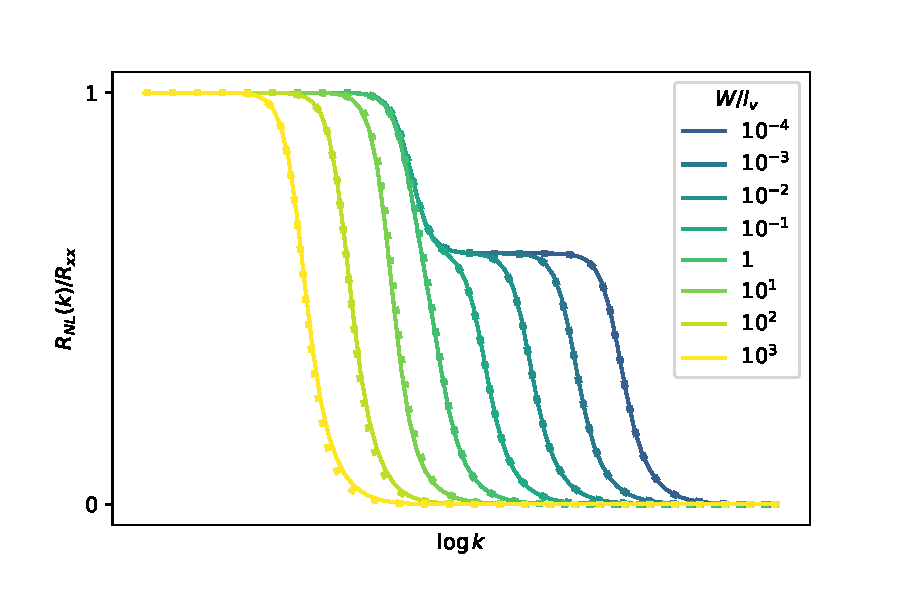
\includegraphics[width=\linewidth]{Immagini/rnl/kapproxcomp.pdf}
    \caption{Comparison between $R_{NL}(k)$ and $\tilde R_{NL}(k)$. The continuous line represents $R_{NL}(k)$, while the dashed line represents $\tilde R_{NL}(k)$}
    \label{fig:kapproxcomp}
\end{figure}\\
The nice thing about this is that if two equations are similar, then their Fourier transform will be too. We can transform $\tilde R_{NL}(k)$ with equations \ref{eq:rxg} and \ref{eq:rxl} and we get that

\begin{equation}
    \boxed{
        \tilde R_{NL}(x)=
        \frac{W \rho_{c,xx}e^{-|x|/L_v}}{2L_v[1+\tan^{-2}(\Theta_{VH})]}-
        \frac{2\rho_{c,xx}}{\pi [1+\tan^2(\Theta_{VH})]}\ln \bigg|\tanh \Big(\frac{\pi x}{2W}\Big)\bigg|
    }
\end{equation}
Infact if we re-create figure \ref{fig:rnlx2approx} with the equation above we get figure \ref{fig:rnlxapprox}

\begin{figure}[h!]
    \centering
    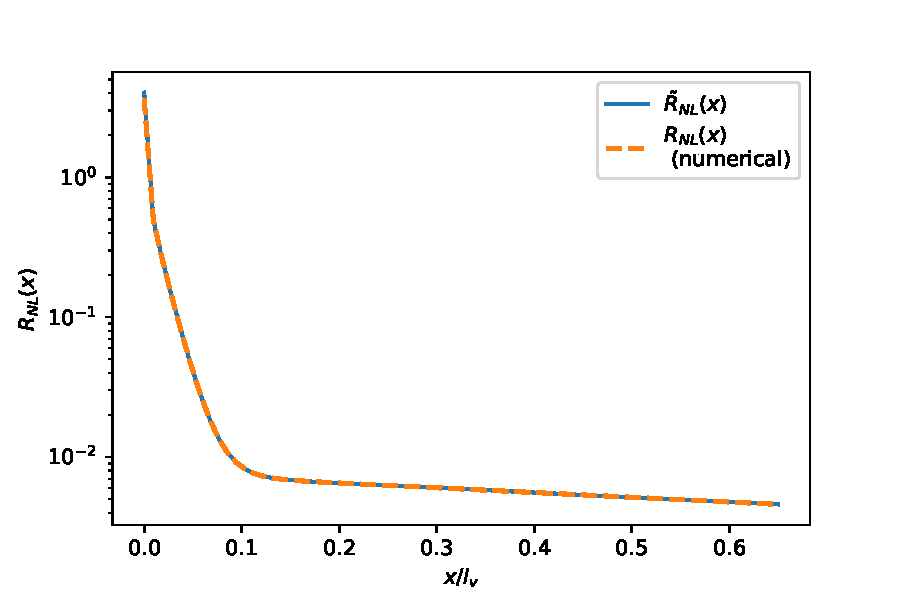
\includegraphics[width=\linewidth]{Immagini/rnl/xapprox.pdf}
    \caption{As you can see it's impossible to distinguish the difference between the two functions to the naked eye. The parameters are the same as figure \ref{fig:rnlxapprox}}
    \label{fig:rnlxapprox}
\end{figure}